\chapter{Dedicação Para a Tese}

\begin{center}

\includegraphics[width=0.5\linewidth]{Images/dedicacao.png}    
\end{center}
\vspace{0.5cm}



\gxatencao{A única maneira de se acabar uma tese é com dedicação.}


Dedicar-se significa reservar horas para seu trabalho de tese. A tese não pode ficar relegada às horas livres, pois essas tendem a sumir rapidamente. 


Dedicar-se significa se esforçar para obter informações, descobrir que informações são necessárias e manter um ritmo de trabalho constante no início e crescente do meio para o final. 


É importante estar preparado para dedicação exclusiva nos dias finais que antecedem a entrega da tese e lembrar de reservar alguns dias para fazer as correções solicitadas pela banca.


A melhor maneira de se dedicar é ter um plano de horários e obedecê-lo, planejar a tese como se fosse um dia de trabalho e cumprir o planejamento. Devo dizer que nunca vi alguém fazer isso, pois as necessidades do dia a dia acabam se encaixando com a flexibilidade dos horários de estudo e “bagunçando o coreto”. Mas aqui vão algumas dicas para organizar sua dedicação:

\begin{outline}
\1	Carga Horária


\2	Determine uma carga horária mínima por dia, por semana e por mês. Tente cumprir todas as cargas horárias. Nunca deixe a carga mínima do mês atrasar.


\1	Metas Específicas


\2	Defina metas específicas, principalmente quando relacionadas à parte do texto da tese e parte do software. Dê um prazo para essas metas. Tenha metas objetivas para cada final de período letivo.


\1	Horário de Trabalho


\2	Defina um horário de trabalho preferido. Você pode ser do tipo madrugador ou noturno. Aproveite a flexibilidade para trabalhar na hora que produz mais. 


\3	Ao longo do tempo, apesar de madrugador, passei a considerar que é mais produtivo que a tese seja seu primeiro trabalho do dia, de modo que você não esteja nem cansado, nem influenciado por outros problemas. Assim, recomendo a meus alunos que têm atividades paralelas acordar pelo menos uma hora mais cedo todo dia para trabalhar na tese.


\1	Aos que dormem tarde, garanto que com o tempo passarão a dormir mais cedo.
\end{outline}

\section{Avaliando Seu Trabalho}


Uma maneira de saber como seu trabalho está andando é avaliá-lo periodicamente. Todo dia se pergunte: eu fiz algo para atingir meu objetivo?


Duas perguntas são importantes em relação aos seus objetivos de tese:

\begin{outline}
\1	O que você escreveu?


\2	Tem relação ao seu trabalho escrevendo capítulos da tese, programas, especificações e artigos em revista. 


\2	Responda à pergunta: em quantos trabalhos desse tipo eu coloquei algum esforço hoje e produzi algum resultado palpável?


\1	Com quem você colaborou?


\2	Tem relação aos tipos de colaborações que você fez nesse dia, semana ou mês. Formas de colaboração possível são:


\3	Fiz algo para meu orientador?


\3	Fiz algo para um colega?


\3	Pedi algo para um colega? 


\3	Dividi algo com um colega?
\end{outline}

\section{Objetivos S.M.A.R.T.}


Um método interessante de criar objetivos em seu trabalho, ou em sua vida em geral, é lembrar do acrônimo S.M.A.R.T. Segundo essa teoria, um objetivo deve ser:

\begin{outline}
\1	S – eSpecífico (Specific)


\2	O objetivo deve ser específico e não generalizado. Ou seja, deve ser algo que pode ser claramente atingido. Um bom exemplo é “entrar em uma academia e me exercitar 3 vezes por semana” e não “malhar”. 


\1	M – Mensurável (Measurable)


\2	Deve ser possível avaliar que ele foi atingido. O exemplo típico é ótimo: “perder 5 quilos”.


\1	A – Atingível (Attainable)


\2	O objetivo tem que ser alcançável. Você tem que se propor a realizá-lo e tem que compreender suas dificuldades.


\1	R – Realista (Realistic)


\2	O objetivo tem que ser realista. Não adianta querer perder 50 quilos em uma semana. 


\1	T – limitado no Tempo (Time Bound)


\2	Você tem que dar um prazo para o objetivo acontecer. Por exemplo “Perder 5 quilos em 3 meses”.


\2	Alguns autores consideram T para “Tangível”, no sentido de ser algo que possa ser avaliado de acordo com os 5 sentidos (tato, paladar, visão, audição e olfato). 
\end{outline}

Relacionados à tese, bons objetivos podem ser:

\begin{itemize}
	\item	Escrever um capítulo de revisão bibliográfica de 15 páginas em um mês.
	
	
	\item	Escrever um artigo descrevendo a experiência realizada até dia 30 de setembro.
	
\end{itemize}


Devemos lembrar que os prazos que recebemos da instituição e de congressos e revistas são ótimos mecanismos para determinar nossos limites no tempo.



\section{Técnicas de Estudo e Trabalho}


Existem muitas maneiras de trabalhar e estudar, principalmente na frente do computador. Quero chamar atenção a uma técnica e uma teoria que são muito difundidas, mas que são opostas, respectivamente, Pomodoro, Flow (ou Fluxo).


Fluxo é uma teoria proposta por Mihaly Csikszenbtmihalyi que diz que existe um estado de alta concentração onde entramos em fluxo. O fluxo é um estado da mente onde estamos altamente focados no trabalho, não sentimos o tempo passar. Para alcançar o fluxo cada pessoa precisa de um certo tempo, que pode chegar a 30 minutos. Porém, se perdemos a concentração, saímos imediatamente do estado de fluxo e voltamos a precisar do mesmo tempo para entrar de novo nele. 


Seguindo esse caminho, é importante reservar momentos mais longos e com nenhuma interrupção. Se desligar do celular e das redes sociais é essencial para atingir o Fluxo.


Pomodoro é uma prática de estudo onde treinamos o cérebro para funcionar focado em curtos períodos. Tradicionalmente se usa 25 de trabalho por 5 de descanso por ciclo, mais 15 a 20 minutos de descanso depois de 3 ciclos. A principal parte dessa técnica é gerenciar as distrações.


Claramente a técnica Pomodoro interrompe o estado de fluxo. Não está claro qual escolher, talvez algumas tarefas sejam adequadas a procurar o fluxo e outras a técnica de Pomodoro. Pessoalmente eu reconheço minha capacidade de entrar em estado de fluxo quando faço tarefas como escrever algo ou programar, conseguindo grande concentração. Confesso que as vezes, ao sair do fluxo, tenho até dificuldade de entender de novo o código que escrevi. Já a técnica Pomodoro não funciona bem comigo, que tenho tendência a procurar desculpas para exceder o tempo de descanso, me envolvendo com outras atividades.


Sugiro aos leitores que se aprofundem mais nas duas técnicas, façam experimentos consigo mesmos e escolham a que mais se adapta ao seu estilo.


\section{Ambiente de Estudo}


Uma das coisas mais importantes é ter um ambiente de estudo onde você se sinta bem. Alguns preferem o silêncio, outros necessitam de música, cada um tem um gosto pessoal. Aqui vão algumas dicas: 

\begin{itemize}
\item	Tenha um computador próprio e exclusivo. 


\item	Lembre-se: você é um aluno de Computação, o mínimo que pode ter é um computador próprio.


\item	Isso também é uma defesa, já que você não quer que outros destruam sem intenção o seu trabalho.


\item	Tenha um ambiente de estudo em casa e um na faculdade. 


\item	Cultive esses ambientes, retirando dele tudo que pode atrapalhar sua concentração e usando-os prioritariamente. 


\item	Em cada início de período dê uma “arrumada” no seu computador, evitando assim problemas graves no meio do período. 


\item	Evite estudar em uma posição que leve ao sono. 


\item	Tenha uma estante reservada para o material de estudo. 


\item	Mantenha seus artigos organizados. Encaderne-os ou coloque-os em fichários, ou em diretórios organizados. Eu uso o software Calibre para todos meus PDFs, por exemplo.
\end{itemize}

\section{O Método do Tadeu}


Um dos alunos mais organizados que tive foi o Tadeu Classe. Ele me mandou esse relato sobre como se organiza.

\begin{quote}
Desde que comecei meu doutorado constantemente vinha percebendo que precisava organizar melhor as minhas tarefas. Sou um doutorando que não faz somente a sua pesquisa, pois preciso me manter na cidade onde vivo, e tenho outras atividades, como treinos esportivos, lecionar em instituições de ensino superior e trabalhar como analista de sistemas.

\begin{figure}[hbt]
	\centering
	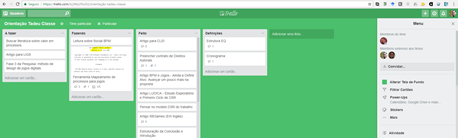
\includegraphics[width=0.7\linewidth]{Images/Trello}
	\caption{Imagem do Trello, software que o Tadeu usou durante sua tese. Fonte: imagem fornecida por Tadeu Classe}
	\label{fig:trello}
\end{figure}

Devido a isso, a minha desorganização vinha tomando conta, e não conseguia desempenhar nenhumas das atividades que realizava com qualidade. Um dos meus orientadores, a Profª. D.Sc. Renata Araujo da UNIRIO, sempre sugeriu desde o início dos meus estudos, que eu tentasse me organizar usando o programa Trello (https://trello.com/), que é um quadro virtual de atividades, onde você consegue organizar e grupos e ir colocando lembretes para a realização das atividades, porém, pessoalmente não gostei muito de usar a ferramenta. Pois mesmo organizando as tarefas, e o que eu precisava fazer, eu não lembrava de acessá-la e atualizá-la.

\begin{figure}[hbt]
	\centering
	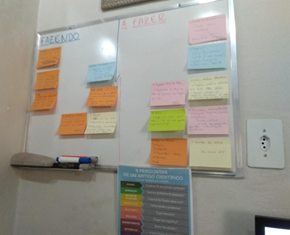
\includegraphics[width=0.7\linewidth]{Images/quadroorganizacao}
	\caption{Quadro de organização de Tadeu Class. Fonte: imagem fornecida por Tadeu Classe.}
	\label{fig:quadroorganizacao}
\end{figure}

Entretanto, me baseando no Trello e para que eu conseguisse organizar melhor os meus afazeres durando meu dia a dia como doutorando, analista de sistemas e professor, decidir colocar em meu escritório de trabalho um quadro branco. Neste quadro eu fiz a sua divisão em duas áreas (“A FAZER” e “FAZENDO”) no qual eu anexo “post-its” com as tarefas que eu preciso realizar [Figura 2], trocando entre os lados as prioridades, sendo que as tarefas que forem sendo realizadas, jogo o post-it no lixo. Meus post-its são coloridos, e cada cor indica o grau de urgência da atividade a ser realizada, por exemplo: laranja: URGÊNCIA, azul: PRECISAM SER FEITOS, rosa: FAZER ASSIM QUE SOBRAR UM TEMPO, amarelo: SEM URGÊNCIA, e verde: UM DIA EU FAÇO.

Desta maneira consegui ter um quadro de tarefas onde consigo organizar tudo o que precisa ser feito em meu dia a dia, com a vantagem de que o mesmo está sempre na minha frente fazendo com que eu sempre esteja olhando para ele. Minha produtividade melhorou muito desde então, e ele me auxiliou a entregar todas as demandas nos prazos corretos.

\end{quote}
